\iffalse

\bibliography{..\\bib\\tex.bib}

\fi

\chapter{对词向量性质的分析}

词向量学习或词向量嵌入在今年能够成为研究热点的原因之一,在于学习到的词向量具有许多很好的性质。其中最引入注意的一条是,这些向量往往能够通过代数运算反映词语间的关系。同时很奇妙地是,在学习词向量或进行词向量嵌入的过程中,实际上是没有对这个性质进行显式地约束或建模的。这种性质很像是词向量学习所获得的一种有价值的副产物。下面我们先对词向量的性质进行介绍,再对为什么会出现这条性质进行分析。

\section{词向量的性质的介绍}

通过词嵌入模型学习得到的词向量往往会携带部分语义或语法的信息,而这部分信息,可以通过代数运算反映出来。如我们在\ref{chap:intro}举的例子,$\vvec[\mbox{man}]-\vvec[\mbox{woman}] \approx \vvec[\mbox{king}] - \vvec[\mbox{queen}]$,$\vvec[\mbox{Chinese}] + \vvec[\mbox{river}] \approx \vvec[\mbox{Yangtze\_River}]$,由于man与woman之间的关系与king与queen之间的关系类似,均在与性别的不同,同时,Chinese+River所表达语义与Yangtze\_River类似,所以我们可以认为通过代数运算,词向量可以体现出语义的关系。另一方面,我们还可以观察到$\vvec[\mbox{best}]-\vvec[\mbox{good}] \approx \vvec[\mbox{highest}] - \vvec[\mbox{high}]$,由于类似的原因,我们认为词向量还可以体现出语法间的关系。

为了进一步验证词向量的这条性质,我们使用\emph{word2vec}发布的工具包,并使用维基百科的英文的语料的前一百万个单词训练了200维的词向量,并用这些词向量进行了验证实验。

\subsection{表示国家与首都的单词间的语义关系}

\begin{longtable}{lcccc}
% 首页表头
\caption[部分国家与其对应首都的中英文名称]{作为示例的部分国家与其对应首都的中英文} \label{tab:CountyCity} \\
\toprule[1.5pt]
国家名 & 国家名的英文 & 首都名 & 首都名的中文\\
\midrule[1pt]
中国	&	china	&	北京	&	beijing\\
俄罗斯	&	russia	&	莫斯科	&	moscow	\\
日本	&	japan	&	东京	&	tokyo	\\
法国	&	france	&	巴黎	&	paris	\\
意大利	&	Italy	&	罗马	&	roma	\\
\endfirsthead

\end{longtable}

在第一个实验中,我们选取了表\ref{tab:CountyCity}中的五个国家和他们的首都,并从学习到的词向量中找出他们所对应的向量。为了便于观察,我们将这些向量的维度使用主成分分析(PCA)的方法降维至2维。如图\ref{fig:county_city}所示,表示国家与其首都对应的词向量之间的向量差是非常相似的。其中,$\vvec_{\mbox{东京}}$与$\vvec_{\mbox{日本}}$的向量差与$\vvec_{\mbox{北京}}$与$\vvec_{\mbox{中国}}$的向量差的相似程度尤其高,这是符合我们对他们之间关系的认知的。同样的现象也发生在$\vvec_{\mbox{巴黎}} - \vvec_{\mbox{法国}}$与$\vvec_{\mbox{罗马}} - \vvec_{\mbox{意大利}}$之间。这些实验说明,词向量确实可以较好得反映词语的部分语义信息。

\begin{figure}
\centering
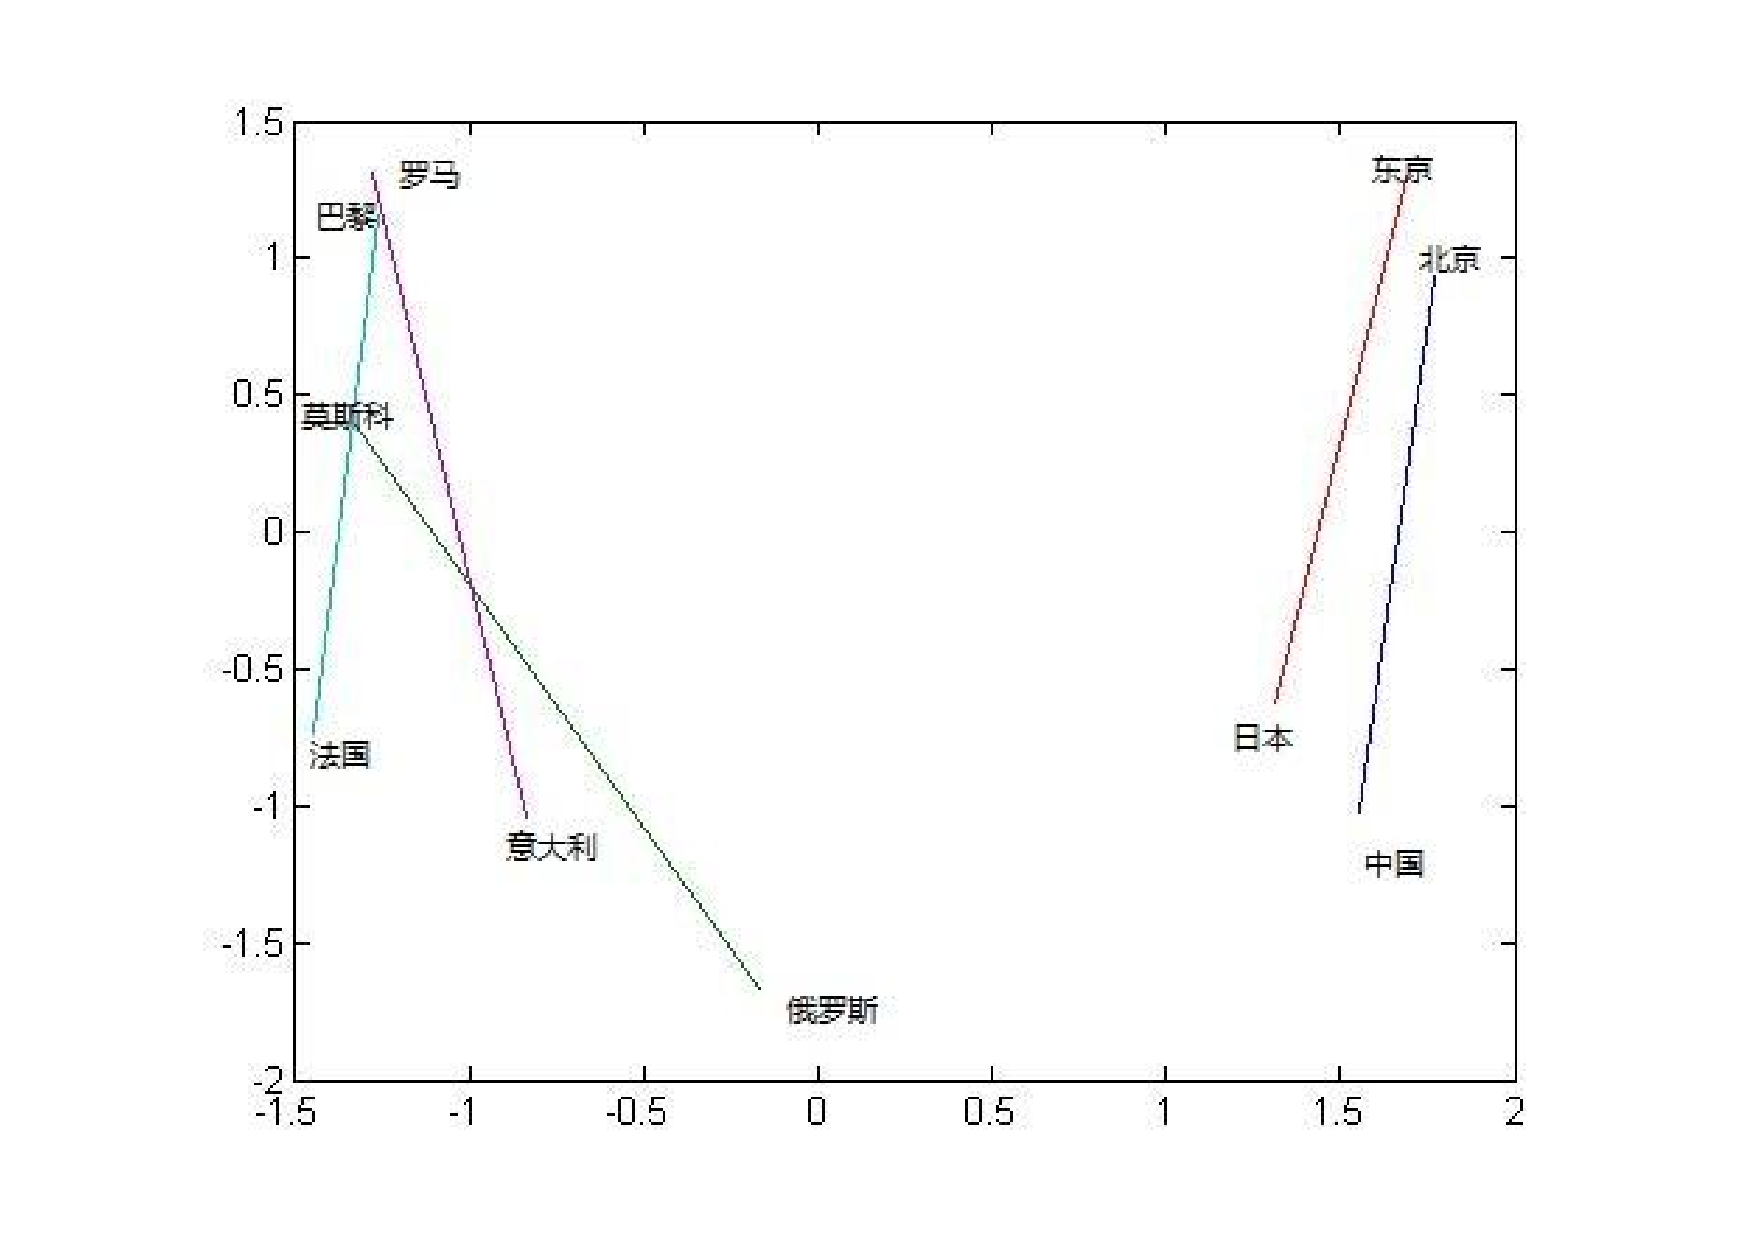
\includegraphics[width=11cm]{county_city}
\caption{5个国家与其首都的降维后的词向量}
\label{fig:county_city}
\end{figure}

\section{对词向量的性质的分析与解释}

在第\ref{chap:w2v}章我们对\emph{word2vec}模型的介绍中,可以发现,\emph{word2vec}模型的假设中并没有涉及到对词向量间代数运算的说明,也无法保证对词向量进行向量加减会得到有意义的结果,可是,实际上,如同我们在上一节所展示的那样,对\emph{word2vec}所学习获得的词向量进行加减,往往是可以获得有意义的结果的。这是为什么呢?我们将在这一节对这一问题进行简单的探讨与分析。

\section{对词向量的差的分析与解释}

\begin{longtable}{lcccc}
% 首页表头
\caption[词语同时出现概率及比例]{在维基百科的前100万单词中统计的到的单词对同时出现概率及其比例} \label{tab:CoProbRatio} \\
\toprule[1.5pt]
概率与比例 & gas & solid & water & fashion\\
\midrule[1pt]
$P(k|ice)$	&$1.504\times10^{-4}$	&$2.406\times10^{-4}$	&$3.248\times10^{-3}$	&$3.008\times10^{-5}$	\\
$P(k|steam)$	&$4.940\times10^{-4}$	&$5.488\times10^{-5}$	&$2.799\times10^{-3}$	&$5.488\times10^{-5}$	\\
$P(k|steam)/P(k|ice)$	&$3.285$	&$0.228$	&$0.862$	&$1.824$	\\
\endfirsthead

\end{longtable}

\cite{pennington2014glove}中提到,对于具有特定关系的一对词语来说,如ice与steam这两个热力学词语,他们之间的关系,可以通过大量的其他词语分别与这两个词语同时出现的概率来确定。如对于ice与steam,我们选取了4个词语,solid,gas,water,fashion,并把他们与ice和steam同时出现的概率及其比率汇总在表\ref{tab:CoProbRatio}。这四个词中,很明显solid和gas是对这两个词有偏向性的(solid更与ice有关而gas更与steam有关),而water与fashion则是与他们间的关系是无关的(water与这两个词都有关系,fashion与这两个词都没关系)。在这种情况下,ice与steam间的关系可以描述为,使得一个东西与gas变得更相关,与solid变得更不相关。另一方面,表格中的内容也恰好反映出了这一关系。即gas与ice和steam同时出现的概率之比远大于1,而solid与ice和steam同时出现的概率之比远小于1,同时water与fashion同ice和steam同时出现的概率之比均约等于1。

基于此,\cite{pennington2014glove}提出可以通过对词语同时出现的比例进行建模,即构造函数使得$f(\vvec_i, \vvec_j, \vvec_k)$并使函数值尽可能逼近$\frac{P(w_i|w_k)}{P(w_j|w_k)}$。最后提出了新的模型并取得了不错的实验结果。在这里,我们更关系的是为什么通过\emph{word2vec}学习得到的词向量间的差可以反映对应词语见的关系,所以我们对\citep{pennington2014glove}所提出模型的细节不做过多讨论,而将注意力放在对\emph{word2vec}模型的解释上。

如上文所说,在某种程度上,$\frac{P(w_i|w_k)}{P(w_j|w_k)}$的对所有的$w_k \in W$的取值可以反映出$w_i$与$w_j$间的关系。同时,对于一个由\emph{word2vec}训练得到的词向量$\vvec$,我们假设\emph{word2vec}模型中通过上下文预测对应词语或通过对应词语预测上下文均可以获得非常准确的结果,即$f(\vvec_i, \vvec_k) \approx P(w_i|w_k)$,此时$\frac{P(w_i|w_k)}{P(w_j|w_k)}\approx \frac{f(\vvec_i, \vvec_k)}{f(\vvec_j, \vvec_k)}$而在\emph{word2vec}的模型中,$f(\vvec_i, \vvec_k) = \frac{e^{{\vvec'_i}^\top\vvec_k}}{\sum_{w_l \in W}e^{{\vvec'_l}^\top\vvec_k}}$,此时有:
\begin{equation*}
\frac{P(w_i|w_k)}{P(w_j|w_k)}\approx e^{({\vvec'_i-\vvec'_j)}^\top\vvec_k}
\end{equation*}
即对于$w_i$与$w_j$,反映它们之间关系的比值可以由他们的对应的词向量的向量差近似得进行逼近。进一步,我们可以说词向量之间的向量差的结果可以表示他们对应词语间的意义。

\section{对词向量的和的分析与解释}

在上一节,我们在\citep{pennington2014glove}中分析的基础上对$\vvec[\mbox{man}]-\vvec[\mbox{woman}] \approx \vvec[\mbox{king}] - \vvec[\mbox{queen}]$的现象出现的原因进行了讨论。下面我们对另外一种向量运算对于词向量的作用,即$\vvec[\mbox{Chinese}] + \vvec[\mbox{river}] \approx \vvec[\mbox{Yangtze\_River}]$现象出现的原因进行讨论。

直观上,加法的意义应该对词义有类似聚合的叠加的效果,例如Yangtze\_River是Chinese的最著名的River,所以他可以视为Chinese与River的语义的叠加。但是为什么有这种现象出现呢?

在我看来,如果$w_i$与$w_j$的语义/语法的叠加可以替代$w_k$,那么,对于$w_k$出现的上下文,如果将$w_k$换成包含$w_i$,$w_j$的序列应该也是符合语义/语法的。换言之,由于$w_k$与$w_i$,$w_j$的序列存在某种等价性,根据上文提到过的\emph{The Distributional Hypothesis},他们的语言环境或上下文应该也存在某种等价性。 这种等价性在\emph{word2vec}中可以表述为:
\begin{equation}
\label{eq:plus1}
P(\mbox{某个上下文env}|w_k) \approx P(\mbox{某个上下文env}|w_iw_j)
\end{equation}

另一方面,根据$w_i$与$w_j$之间独立的假设,我们有:
\begin{eqnarray*}
P(\mbox{某个上下文env}|w_iw_j) &=& P(\vvec_{env}|w_iw_j)\\
&=& \frac{\frac{e^{(\vvec'_i+\vvec'_j)^\top \vvec_{env}}}{ (\sum_{w_l \in W} e^{{\vvec'_l}^\top\vvec_{env}})^2} \cdot P(\vvec_{env}) } { \sum_{w_m \in W}{\frac{e^{(\vvec'_i+\vvec'_j)^\top \vvec_m}}{ (\sum_{w_l \in W} e^{{\vvec'_l}^\top\vvec_m})^2} \cdot P(\vvec_m)} }
\end{eqnarray*}
其中,$P(\vvec_m)$表示$w_m$出现的概率,我们可以假设他近似满足条件:
\begin{equation*}
P(\vvec_m) \propto (\sum_{w_l \in W} e^{{\vvec'_l}^\top\vvec_m})^2 
\end{equation*}
此时,我们可以得到$P(\mbox{某个上下文env}|w_iw_j)$的一个近似:
\begin{equation}
\label{eq:plus2}
P(\mbox{某个上下文env}|w_iw_j) \approx \frac{e^{(\vvec'_i+\vvec'_j)^\top \vvec_{env}}}{\sum_{w_m \in W} e^{(\vvec'_i+\vvec'_j)^\top \vvec_m}}
\end{equation}

同时,$P(\mbox{某个上下文env}|w_k)$在\emph{word2vec}中有类似的形式,即:
\begin{equation}
\label{eq:plus3}
P(\mbox{某个上下文env}|w_k) = \frac{e^{{\vvec'_k}^\top \vvec_{env}}}{\sum_{w_m \in W} e^{{\vvec'_k}^\top \vvec_m}}
\end{equation}

由式\ref{eq:plus2},式\ref{eq:plus1},式\ref{eq:plus3}我们知道,如果$w_i$,$w_j$的序列与$w_k$存在某种等价,则会导致$P(\mbox{某个上下文env}|w_k) \approx P(\mbox{某个上下文env}|w_iw_j)$。进一步,基于我们对这个概率的假设,会导致$\vvec_i + \vvec_j \approx \vvec_k$,即词向量的和可以表示语义的叠加。